\newenvironment*{dummyenv}{}{}

\subsection{应用举例}\label{subsec:15-10}

下面举例说明解斜三角形在实际中的一些应用。

\liti 自动卸货汽车的车箱采用液压机构。设计时需要计算油泵顶杆 $BC$ 的长度(图 \ref{fig:15-26})。
已知车箱的最大仰角为 $60^\circ$,油泵顶点 $B$ 与车箱支点 $A$ 之间的距离为 $1.95$ 米,
$AB$ 与水平线之间的夹角为 $6^\circ20'$,$AC$ 长为 $1$ 米,计算 $BC$ 的长(保留三个有效数字)。

\begin{figure}[htbp]
    \centering
    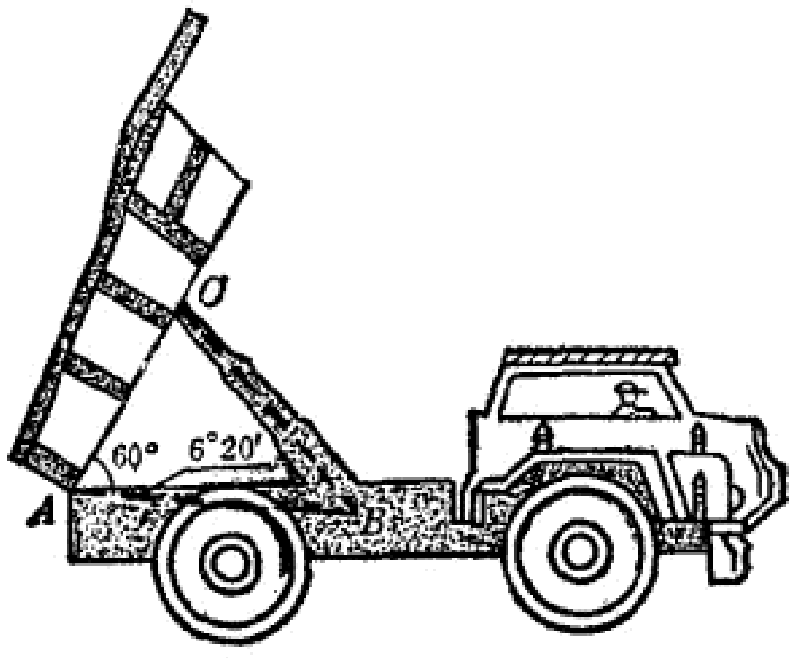
\includegraphics[width=0.5\textwidth]{../pic/czds4-ch15-26}
    \caption{}\label{fig:15-26}
\end{figure}

分析:这个问题就是在 $\triangle ABC$ 中,已知 $AB = 1.95$ 米,$AC = 1.40$ 米,
$\angle BAC = 60^\circ +  6^\circ20' = 66^\circ20'$,求 $BC$ 的长。
由于已知 $\triangle ABC$ 的两边和一夹角,所以可根据余弦定理求出 $BC$。

\jie 由余弦定理

$\begin{aligned}
    BC^2 &= AB^2 + AC^2 - 2 AB \cdot AC \cos{A} \\
         &= 1.95^2 + 1.40^2 - 2 \times 1.95 \times 1.40 \times \cos{66^\circ20'} \juhao
\end{aligned}$

设 $u = 2 \times 1.95 \times 1.40 \times \cos{66^\circ20'}$,

两边取对数,查表并计算,得
\begin{align*}
    \lg{u} &= \lg{2} + \lg{1.95} + \lg{1.40} + \lg{\cos{66^\circ20'}} \\
           &= 0.3010 + 0.2900 + 0.1461 + \overline{1}.6036 \\
           &= 0.3407 \douhao
\end{align*}

查反对数表得
$$ u = 2.192 \juhao $$

$\therefore$ \quad $\begin{aligned}[t]
    BC^2 &= 1.95^2 + 1.40^2 - 2.192 \\
         &= 3.803 + 1.960 - 2.192 \\
         &= 3.571 \douhao
\end{aligned}$

查平方根表得
$$ BC = 1.889 \approx 1.89 \; (\mi) \juhao $$

答:顶杆 $BC$ 约长 $1.89$ 米。


\begin{wrapfigure}[10]{r}{7cm}
    \centering
    \begin{tikzpicture}[
    river/.style={decorate, decoration={random steps,segment length=3pt,amplitude=2pt}},
    scale=0.8,
]
    \pgfmathsetmacro{\factor}{0.06}
    \pgfmathsetmacro{\bc}{78.35 * \factor}
    \pgfmathsetmacro{\jiaob}{69.717} % 69度43分
    % \pgfmathsetmacro{\jiaoc}{41.2}   % 41度12分
    \pgfmathsetmacro{\ab}{55.26 * \factor}
    \coordinate (B) at (0, 0);
    \coordinate (C) at (\bc, 0);
    \coordinate (A) at (\jiaob:\ab);
    \draw [thick] (B) node [left] {$B$} -- (C) node [right] {$C$};
    \draw [dashed] (B) -- (A) node [above] {$A$} -- (C);
    \draw pic [draw, angle radius=0.8em] {angle=C--B--A};
    \draw pic [draw, angle radius=0.8em] {angle=A--C--B};

    \begin{scope}[xshift=2cm, yshift=8.5cm]
        \foreach \x in {1, ..., 4, 7, 8, 9, 10} {
            \pgfmathsetmacro{\r}{6 + \x/5}
            \draw [river] (240:\r) arc (240:300:\r);
        }
    \end{scope}
\end{tikzpicture}


    \caption{}\label{fig:15-27}
\end{wrapfigure}

\liti 为了在一条河上建一座桥,施工前在河两岸打上两个桥位桩 $A$, $B$(图 \ref{fig:15-27})。
要精确测算出 $A$, $B$ 两点间的距离,测量人员在岸边定出基线 $BC$,测得 $BC = 78.35$ 米,
角 $B = 69^\circ43'$, 角 $C = 41^\circ12'$,计算 $AB$ 的长(精确到 $0.01$ 米)。

\jie 在 $\triangle ABC$ 中,已知 $a = 78.35$, $B = 69^\circ43'$, $C = 41^\circ12'$。

$A = 180^\circ - (B + C) = 180^\circ - (69^\circ43' + 41^\circ12') = 69^\circ5'$。

由正弦定理,可得
$$ c = \dfrac{a \sin{C}}{\sin{A}} \juhao $$

两边取对数,查表并计算,得
\begin{align*}
    \lg{c} &= \lg{a} + \lg{\sin{C}} - \lg{\sin{A}} \\
           &= \lg{78.35} + \lg{\sin{41^\circ12'}} - \lg{\sin{69^\circ5'}} \\
           &= 1.8941 + \overline{1}.8187 - \overline{1}.9704 \\
           &= 1.7424 \juhao
\end{align*}

查反对数表得
$$ c = 55.26 \; (\mi) \juhao $$

答:桥位桩 $A$、$B$ 间的距离约为 $55.26$ 米。


\begin{dummyenv}
\renewcommand{\haomi}{\mathord{\text{mm}}}%毫米

\liti 图 \ref{fig:15-28} 是曲柄连杆机构的示意图。当曲柄 $CB$ 绕 $C$ 点旋转时,
通过连杆 $AB$ 的传递,使活塞作直线往复运动。
当曲在 $CB_0$ 位置时,曲柄和连杆成一条直线,连杆的端点 $A$ 在 $A_0$ 处。
设连杆 $AB$ 长 $340$ mm,曲柄 $CB$ 长 $85$ mm,
求曲柄自 $CB_0$ 按顺时针方向旋转 $80^\circ$ 时,活塞移动的距离
(即连杆的端点 $A$ 移动的距离 $A_0A$)(精确到 $1$ mm)。

\begin{figure}[htbp]
    \centering
    \begin{minipage}[b]{8cm}
        \centering
        \begin{tikzpicture}[
    every node/.style={fill=white, inner sep=1pt, outer sep=2pt},
]
    \pgfmathsetmacro{\factor}{0.01}
    \pgfmathsetmacro{\ab}{340 * \factor}
    \pgfmathsetmacro{\bc}{85 * \factor}
    \pgfmathsetmacro{\aa}{81 * \factor} %AA_0
    \pgfmathsetmacro{\r}{0.12}      % A、B、C 点小圆圈的半径
    \pgfmathsetmacro{\R}{0.24}      % A、B、C 点(不完整的)大圆圈的半径
    \pgfmathsetmacro{\z}{20}        % A、B、C 点(不完整的)大圆圈缺口的偏移度数
    \pgfmathsetmacro{\jiaoa}{14.25} % A=14度15分

    \coordinate ["$A_0$" below] (A0) at (0, 0);
    \coordinate ["$B_0$" below left] (B0) at (\ab, 0);
    \coordinate ["$C$" {below, yshift=-0.5em}] (C)  at (\ab + \bc, 0);
    \coordinate ["$B$" {above, yshift=0.5em}] (B)  at ($(C) + (100:\bc)$);
    \coordinate ["$A$" {right, xshift=0.2em, yshift=-0.2em}] (A)  at (\aa, 0);

    \draw pic [draw, "\tiny $80^\circ$", angle radius=1.2em, angle eccentricity=1] {angle=B--C--A};
    \filldraw [fill=black] (A0) circle (0.05);
    \draw [densely dash dot] (-1.2, 0) -- (5.5, 0);
    \draw [densely dash dot] (B) -- (C);
    \draw [dashed] (C) circle (\bc);
    \draw (C) circle (\r);
    \draw (C) + (100+\z:\R) coordinate (X1)
        arc (100+\z:360+100-\z:\R) coordinate (X2);
    \draw (B) circle (\r);
    \draw [name path=circle b] (B) + (280+\z:\R) coordinate (X4)
        arc (280+\z:360+280-\z:\R) coordinate (X3);
    \draw (X1) -- (X3) (X2) -- (X4);

    \draw [densely dash dot] (A) -- (B);
    \draw (A) circle (\r);
    \draw (A) + (\jiaoa+\z:\R) coordinate (X5)
        arc (\jiaoa+\z:360+\jiaoa-\z:\R) coordinate (X6);
    \path [name path=x5] (X5) -- +(\jiaoa:\ab-\R);
    \path [name path=x6] (X6) -- +(\jiaoa:\ab-\R);
    \draw [name intersections={of=x5 and circle b, by=X7}] (X5) -- (X7);
    \draw [name intersections={of=x6 and circle b, by=X8}] (X6) -- (X8);

    %---------------------- 绘制带阴影的部件----------------------------------------------------------
    \begin{scope}
        % 从左到右: xa, xb, xc, ...
        % 从下到上: ya, yb, yc, ...
        \pgfmathsetmacro{\d}{0.2}    % 阴影部分的宽度
        \pgfmathsetmacro{\h}{1}      % “L” 型部件的高度
        \pgfmathsetmacro{\pa}{-0.7}  % 定义三个不同的位置
        \pgfmathsetmacro{\pb}{-0.3}
        \pgfmathsetmacro{\pc}{2}

        \begin{scope} % 靠近 A 点的 “[” 型部件
            \pgfmathsetmacro{\xb}{\aa - \R}
            \pgfmathsetmacro{\xa}{\xb - \d}
            \pgfmathsetmacro{\xc}{\xb + 2 * \R + 0.2}
            \pgfmathsetmacro{\yb}{0 - \R}
            \pgfmathsetmacro{\ya}{\yb - \d}
            \pgfmathsetmacro{\yc}{0 + \R + 0.1}
            \pgfmathsetmacro{\yd}{\yc + \d}

            \draw [thick, pattern={mylines[angle=45, distance={5pt}]}]
                (\xa, \ya) -- (\xa, \yd) -- (\xc, \yd) -- (\xc, \yc)
                -- (\xb, \yc) -- (\xb, \yb) -- (\xc, \yb) -- (\xc, \ya)
                -- cycle;
        \end{scope}

        \begin{scope} % “[” 型部件上、下方的 “L” 型部件
            \pgfmathsetmacro{\xa}{\pb}
            \pgfmathsetmacro{\xb}{\xa + \d}
            \pgfmathsetmacro{\xc}{\pc}

            \begin{scope} % 上方的 “L” 型部件
                \pgfmathsetmacro{\ya}{0 + \R + 0.1 + \d} % "["部件上边
                \pgfmathsetmacro{\yb}{\ya + \d}
                \pgfmathsetmacro{\yc}{\ya + \h}

                \path [pattern={mylines[angle=45, distance={5pt}]}]
                    (\xb, \yc) -- (\xb, \yb)
                    -- (\xc, \yb) -- (\xc, \ya)
                    -- (\xa, \ya) -- (\xa, \yc)
                    -- cycle;
                \draw [thick]
                    (\xb, \yc) -- (\xb, \yb)
                    -- (\xc, \yb) -- (\xc, \ya)
                    -- (\xa, \ya) -- (\xa, \yc);
            \end{scope}

            \begin{scope} % 下方的 “L” 型部件
                \pgfmathsetmacro{\yc}{0 - \R - \d} % "["部件下边
                \pgfmathsetmacro{\yb}{\yc - \d}
                \pgfmathsetmacro{\ya}{\yc - \h}

                \path [pattern={mylines[angle=45, distance={5pt}]}]
                    (\xa, \ya) -- (\xa, \yc)
                    -- (\xc, \yc) -- (\xc, \yb)
                    -- (\xb, \yb) -- (\xb, \ya)
                    -- cycle;
                \draw [thick]
                    (\xa, \ya) -- (\xa, \yc)
                    -- (\xc, \yc) -- (\xc, \yb)
                    -- (\xb, \yb) -- (\xb, \ya);
            \end{scope}
        \end{scope}

        \begin{scope} % “[” 型部件左侧的 “(” 型部件
            \pgfmathsetmacro{\xa}{\pa}
            \pgfmathsetmacro{\xb}{\xa - \d}
            \pgfmathsetmacro{\yb}{0 - \R - \d} % "["部件下边
            \pgfmathsetmacro{\ya}{\yb - \h}
            \pgfmathsetmacro{\yc}{0 + \R + 0.1 + \d} % "["部件上边
            \pgfmathsetmacro{\yd}{\yc + \h}
            \path [pattern={mylines[angle=45, distance={5pt}]}]
                (\xa, \ya) -- (\xa, \yb) to [out=115,in=245] (\xa, \yc) -- (\xa, \yd)
                -- (\xb, \yd) -- (\xb, \yc) to [out=245, in=115] (\xb, \yb) -- (\xb, \ya)
                -- cycle;
            \draw [thick]
                (\xa, \ya) -- (\xa, \yb) to [out=115,in=245] (\xa, \yc) -- (\xa, \yd)
                (\xb, \ya) -- (\xb, \yb) to [out=115,in=245] (\xb, \yc) -- (\xb, \yd);
        \end{scope}
    \end{scope}

\end{tikzpicture}


        \caption*{(1)}
    \end{minipage}
    \qquad
    \begin{minipage}[b]{6cm}
        \centering
        \begin{tikzpicture}
    \pgfmathsetmacro{\factor}{0.01}
    \pgfmathsetmacro{\ab}{340 * \factor}
    \pgfmathsetmacro{\bc}{85 * \factor}
    \pgfmathsetmacro{\aa}{81 * \factor} %AA_0

    \coordinate (A0) at (0, 0);
    \coordinate (B0) at (\ab, 0);
    \coordinate (C)  at (\ab + \bc, 0);
    \coordinate (B)  at ($(C) + (100:\bc)$);
    \coordinate (A)  at (\aa, 0);

    \draw (A0) node[below=0.5em] {$A_0$} -- (C) node [below] {$C$};
    \draw (A) node [below=0.5em] {$A$}   -- (B) node [above] {$B$};
    \draw (C) circle (\bc) -- (B);
    \draw pic [draw, "$80^\circ$" {xshift=-0.7em, yshift=0.5em}, angle radius=0.8em] {angle=B--C--A};
    \draw (B0) node [below left] {$B_0$};
    \foreach \x in {A0, A} {
        \draw (\x) +(0, 0.3em) -- +(0, -0.3em);
    }

    % 添加占位用的 path,这样,显示时,两个图的 x 轴(直线AC)在同一水平位置
    \pgfmathsetmacro{\R}{0.24}      % A、B、C 点(不完整的)大圆圈的半径
    \pgfmathsetmacro{\d}{0.2}    % 阴影部分的宽度
    \pgfmathsetmacro{\h}{1}      % “L” 型部件的高度
    \pgfmathsetmacro{\yabove}{0 + \R + 0.1 + \d} % "["部件下边
    \pgfmathsetmacro{\ybelow}{0 - \R - \d} % "["部件下边
    \path (0, \yabove + \h) -- (0, \ybelow -\h);
\end{tikzpicture}


        \caption*{(2)}
    \end{minipage}
    \caption{}\label{fig:15-28}
\end{figure}



分析:因为 $A_0A = A_0C - AC$,又知 $A_0C = AB + BC = 340 + 85 = 425 (\haomi)$,
所以只要求出 $AC$ 的长,问题就解决了。
在 $\triangle ABC$ 中,已知两边和其中一边的对角,可以由正弦定理求出 $AC$。

\jie 在 $\triangle ABC$ 中,由正弦定理可得
$$ \sin{A} = \dfrac{BC \sin{C}}{AB} \juhao $$

两边取对数,查表并计算,得
\begin{align*}
    \lg{\sin{A}} &= \lg{BC} + \lg{\sin{C}} - \lg{AB} \\
                 &= \lg{85} + \lg{\sin{80^\circ}} - \lg{340} \\
                 &= 1.9294 + \overline{1}.9934 - 2.5315 \\
                 &= \overline{1}.3913 \juhao
\end{align*}

因为 $BC < AB$,所以角 $A$ 为锐角,查表可得
$$ A = 14^\circ15' \juhao $$

$\therefore$ \quad $\begin{aligned}[t]
    B &= 180^\circ - (A + C) \\
      &= 180^\circ - (14^\circ15' + 80^\circ) \\
      &= 85^\circ45' \juhao
\end{aligned}$

再由正弦定理,可得
$$ AC = \dfrac{AC \sin{B}}{\sin{C}} \juhao $$

两边取对数,查表并计算,得
\begin{align*}
    \lg{AC} &= \lg{AB} + \lg{\sin{B}} - \lg{\sin{C}} \\
            &= \lg{340} + \lg{\sin{85^\circ45'}} - \lg{\sin{80^\circ}} \\
            &= 2.5315 + \overline{1}.9988 - \overline{1}.9934 \\
            &= 2.5369 \juhao
\end{align*}

查反对数表得,得
$$ AC = 344.3 \; (\haomi) \juhao $$

因此,$\begin{aligned}[t]
    A_0A &= A_0C - AC = (AB + BC) - AC \\
         &= (340 + 85) - 344.3 \\
         &= 80.7 \approx 81 \; (\haomi) \juhao
\end{aligned}$

答:曲柄自 $CB_0$ 转 $80^\circ$ 时,活塞移动的距离约为 $81$ mm。
\end{dummyenv}


\lianxi
\begin{xiaotis}

\xiaoti{如图,为了测量两点 $A$, $B$(这两点之间不能相互看到,也不能直达)间的距离,
    在地面上选择适当的点 $C$,测得 $AC = 213.4$ 米, $BC = 252.1$ 米,
    $\angle ACB = 50^\circ13'$。计算 $AB$ 的长。
}


\begin{figure}[htbp]
    \centering
    \begin{minipage}[b]{8cm}
        \centering
        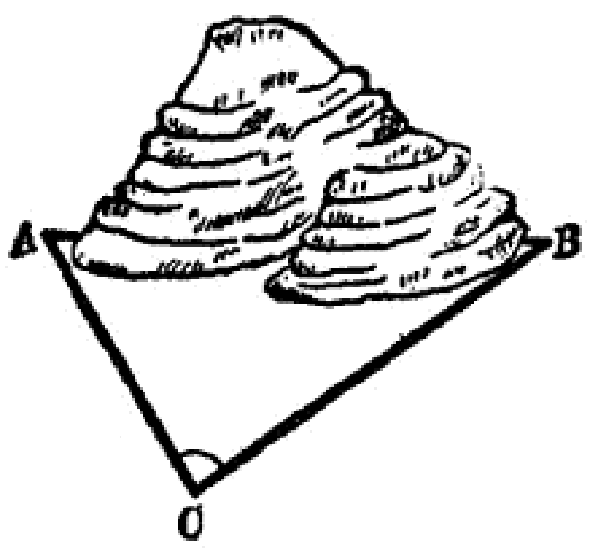
\includegraphics[width=0.6\textwidth]{../pic/czds4-ch15-subsec10-lianxi-1}
        \caption*{(第 1 题)}
    \end{minipage}
    \qquad
    \begin{minipage}[b]{6cm}
        \centering
        \begin{tikzpicture}[>=Stealth, scale=0.8]
    \pgfmathsetmacro{\factor}{0.04}
    \pgfmathsetmacro{\ab}{112.5 * \factor}
    %\pgfmathsetmacro{\bc}{75.4  * \factor}
    \pgfmathsetmacro{\x}{23.56  * \factor}
    \pgfmathsetmacro{\y}{71.62  * \factor}
    \pgfmathsetmacro{\angleb}{atan(\y/\x)}

    \coordinate (B) at (0, 0);
    \coordinate (A) at (\ab, 0);
    \coordinate (C) at (\x, \y);
    \coordinate (D) at (\x, 0);
    \pgfmathsetmacro{\r}{0.4}
    \pgfmathsetmacro{\R}{0.6}
    \pgfmathsetmacro{\RR}{1.1}

    \draw [thick] (A) node [above=1.2em] {\small $A$} circle (\r);
    \draw [thick] (B) node [above=1.2em] {\small $B$} circle (\r);
    \draw [thick] (C) node [above] {\small $C$} circle (\R);

    \path (C) +(45:\RR)  coordinate(pc);
    \path (B) +(165:\RR) coordinate(pb);
    \path (A) +(285:\RR) coordinate(pa);

    \draw [dashed] (A) -- (B) -- (C) -- cycle;
    \draw [dashed] (C) -- (D) node [midway, right] {$y$}
        pic [draw, solid, angle radius=0.5em] {right angle=C--D--A};
    \draw ($(B)!0.6!(D)$) node [above] {$x$};

    \draw [rounded corners] (pc)
        arc [radius=\RR, start angle=45,  end angle=165]
        -- (pb)
        arc [radius=\RR, start angle=165, end angle=285]
        -- (pa)
        arc [radius=\RR, start angle=285, end angle=405]
        -- (pc);
\end{tikzpicture}


        \caption*{(第 2 题)}
    \end{minipage}
\end{figure}


\xiaoti{如图,某零件要镗三个孔 $A$,$B$,$C$,已知孔心距 $AB = 112.5$ mm,
    $BC = 75.4$ mm, $AC = 114.2$ mm。 如果 $A$,$B$ 两孔已加工完毕,
    刀杆在 $B$ 孔处,刀杆要沿 $BA$ 方向和垂直于 $BA$ 方向各移动多少毫米
    (即求 $x$ 和 $y$,确到 $0.1$ mm),才能镗出 $C$ 孔?
}


\xiaoti{如图,要测底部不能到达的烟囱的高 $AB$,从与烟囱底部在同一水平直线上的 $C$, $D$ 两处,
    测得烟囟的仰角分别是 $\alpha = 35^\circ12'$ 和 $\beta = 49^\circ28'$,
    $CD$ 间的距离是 $11.12$ 米。已知测角仪器高 $1.52$ 米,求烟囱的高。
}

\begin{figure}[htbp]
    \centering
    \begin{minipage}[b]{8cm}
        \centering
        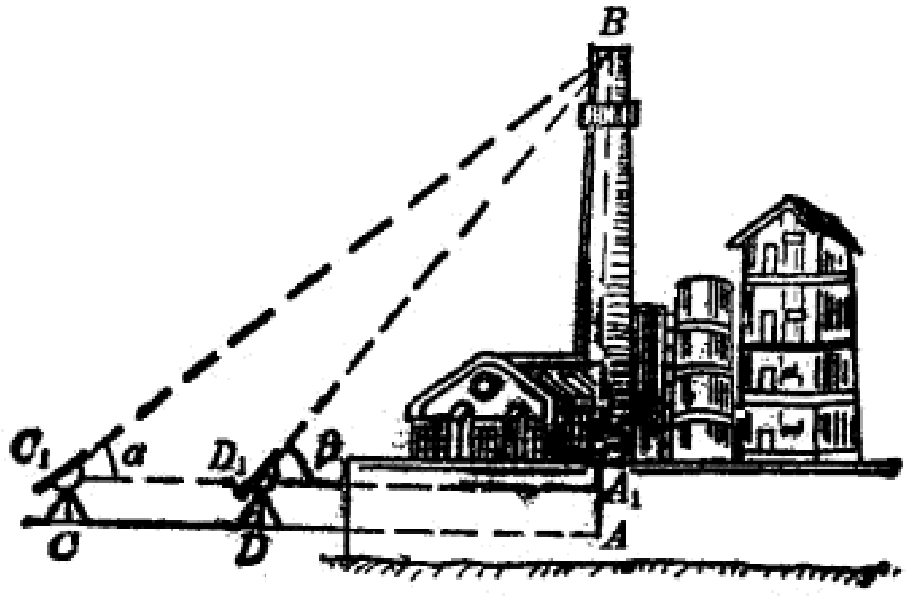
\includegraphics[width=0.9\textwidth]{../pic/czds4-ch15-subsec10-lianxi-3}
        \caption*{(第 3 题)}
    \end{minipage}
    \qquad
    \begin{minipage}[b]{6cm}
        \centering
        \begin{tikzpicture}[>=Stealth,]
    \pgfmathsetmacro{\r}{0.8}
    \coordinate ["$Q$" {below, yshift=-0.3em}] (Q) at (0, 0);
    \coordinate ["$P$" {below, yshift=-0.3em}] (P) at (1, 0);
    \coordinate ["$B$" {below, xshift=-0.5em}] (B) at (3.5, 0);
    \coordinate ["$O$" below] (O) at ($(B) + (\r, 0)$);
    \coordinate ["$A$" above] (A) at ($(O) + (60:\r)$);

    \draw (Q) -- (O) -- (A) -- (P);
    \draw [dashed] (O) circle (\r);
    \draw pic [draw, <-, "$\alpha$" {xshift=-0.7em, yshift=0.5em}, angle radius=0.8em] {angle=A--O--B};
    \foreach \x in {Q, P} {
        \draw [fill=black] (\x) +(-0.5em, -0.3em) rectangle +(0.5em, 0.3em);
    }
    \draw [<->] ([yshift=1.0em] Q) to [xianduan={below=1.0em}] node [above] {$x$} ([yshift=1.0em] P);
\end{tikzpicture}


        \caption*{(第 4 题)}
    \end{minipage}
\end{figure}


\xiaoti{图为曲柄连杆机构示意图。当曲柄 $OA$ 在水平位置 $OB$ 时,连杆端点 $P$ 在 $Q$ 的位置。
    当 $OA$ 自 $OB$ 按顺时针方向旋转 $\alpha$ 角时,$P$ 和 $Q$ 之间的距离是 $x$。
    已知 $OA = 25$ cm, $AP = 125$ cm,求在下列条件下的 $x$ 值(精确到 $0.1$ cm):
}
\begin{xiaoxiaotis}

    \begin{tblr}{columns={18em, colsep=0pt}}
        \xxt{$\alpha = 50^\circ$;} & \xxt{$\alpha = 90^\circ$;} \\
        \xxt{$\alpha = 135^\circ$;} & \xxt{$OA \perp AP$。}
    \end{tblr}
\end{xiaoxiaotis}

\end{xiaotis}
